\chapter{An attempt at Reinforcement Learning of Policies}
\section{Grid World tabular solutions}
In this section, for the sake of example, we assume that a dictionary with 4 key-value pais is less interpretable than a depth-1 decision tree.
In Figure~\ref{fig:optimal-policy}, we illustrate \textit{a}--there are others--tabular optimal policy for the grid world MDP described in the previous section, i.e. that maximizes the objective (cite). 
In any starting state, the agent will move towards the abosrbing state with positive reward.
\begin{figure}[ht]
\centering
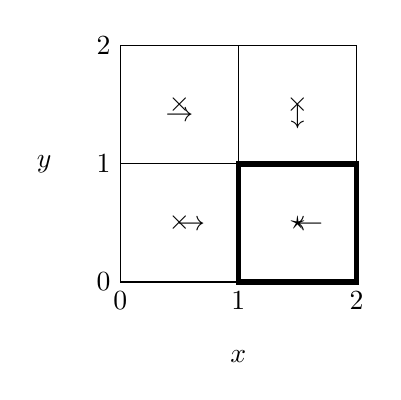
\begin{tikzpicture}[scale=1.5]
    % Draw the grid cells
    \draw (0,0) grid (2,2);
    
    % Add ticks on axes
    \foreach \x in {0,1,2}
        \node[below] at (\x,0) {$\x$};
    \foreach \y in {0,1,2}
        \node[left] at (0,\y) {$\y$};
    
    \node[left] at (-0.5, 1) {$y$};
    \node[below] at (1, -0.5) {$x$};
    
    % Label cells
    \node at (0.5,0.5) {$\times$};
    \node at (0.6,0.48) {$\rightarrow$};

    \node at (0.5,1.5) {$\times$};
    \node at (0.5,1.4) {$\rightarrow$};

    \node at (1.5,1.5) {$\times$};
    \node at (1.5,1.4) {$\downarrow$};
    
    % Goal state in bottom right with double border
    \draw[line width=2pt] (1,0) rectangle (2,1);
    \node at (1.5,0.5) {$\star$};
    \node at (1.6,0.48) {$\leftarrow$};

    
\end{tikzpicture}
\caption{An optimal tabular policy for the grid world.}\label{fig:optimal-policy}
\end{figure}


\begin{figure}[htbp]
    \centering
    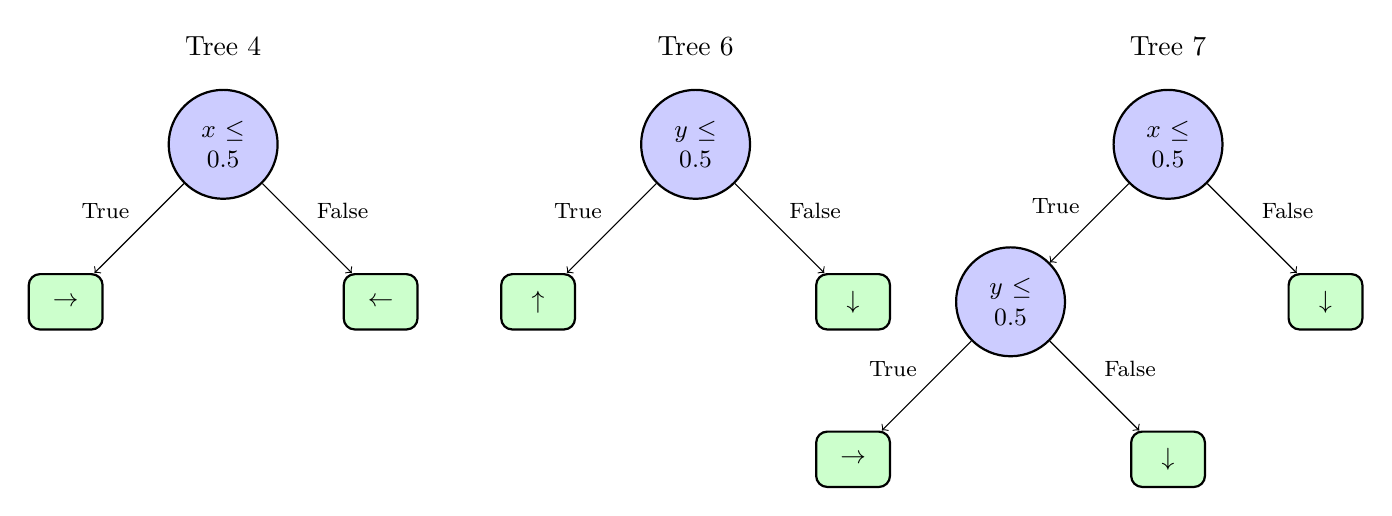
\begin{tikzpicture}[
        scale=1.0,
        decision/.style={circle, draw, thick, fill=blue!20, text width=2.5em, text centered, minimum height=2.5em, font=\small},
        leaf/.style={rectangle, draw, thick, fill=green!20, text width=2em, text centered, rounded corners, minimum height=2em, font=\small},
        edge_label/.style={font=\footnotesize, midway}
    ]
        % Tree 4: if x <= 0.5 move right else move left
        \node[decision] (tree4_root) at (0,0) {$x \leq 0.5$};
        \node[leaf] (tree4_right) at (-2,-2) {$\rightarrow$};
        \node[leaf] (tree4_left) at (2,-2) {$\leftarrow$};
        \draw[->] (tree4_root) -- (tree4_right) node[edge_label, above left] {True};
        \draw[->] (tree4_root) -- (tree4_left) node[edge_label, above right] {False};

        % Tree 6: if y <= 0.5 move up else move down
        \node[decision] (tree6_root) at (6,0) {$y \leq 0.5$};
        \node[leaf] (tree6_up) at (4,-2) {$\uparrow$};
        \node[leaf] (tree6_down) at (8,-2) {$\downarrow$};
        \draw[->] (tree6_root) -- (tree6_up) node[edge_label, above left] {True};
        \draw[->] (tree6_root) -- (tree6_down) node[edge_label, above right] {False};

        % Tree 7: if x <= 0.5 and y <= 0.5 move right else move down
        \node[decision] (tree7_root) at (12,0) {$x \leq 0.5$};
        \node[decision] (tree7_y) at (10,-2) {$y \leq 0.5$};
        \node[leaf] (tree7_right) at (8,-4) {$\rightarrow$};
        \node[leaf] (tree7_down) at (12,-4) {$\downarrow$};
        \node[leaf] (tree7_down2) at (14,-2) {$\downarrow$};
        \draw[->] (tree7_root) -- (tree7_y) node[edge_label, above left] {True};
        \draw[->] (tree7_root) -- (tree7_down2) node[edge_label, above right] {False};
        \draw[->] (tree7_y) -- (tree7_right) node[edge_label, above left] {True};
        \draw[->] (tree7_y) -- (tree7_down) node[edge_label, above right] {False};

        % Labels
        \node[above] at (0,1) {Tree 4};
        \node[above] at (6,1) {Tree 6};
        \node[above] at (12,1) {Tree 7};
    \end{tikzpicture}
    \caption{Some optimal decision tree policies.}
    \label{fig:optimal-policy-trees}
\end{figure}

For this grid world, there exist \textit{optimal} decision tree policies. 
In particular Tree 4 and 6 are have very good interpretability-performance trade-offs (smallest tree that can get the maximum MDP reward).
In the rest of this section we shall attempt to \textit{learn} those trees from data. 


\begin{figure}[htbp]
    \centering
    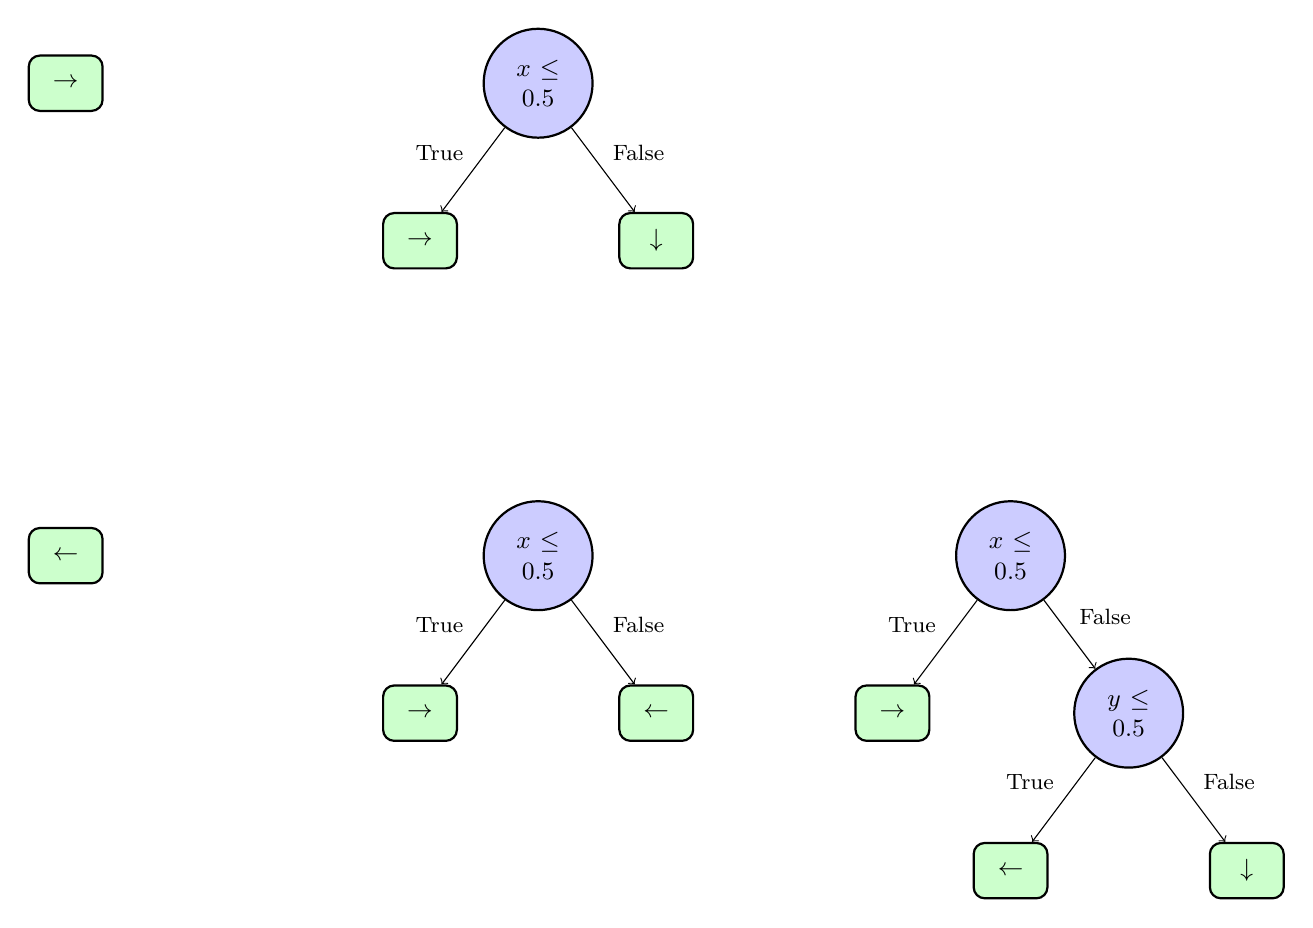
\begin{tikzpicture}[
        scale=1.0,
        decision/.style={circle, draw, thick, fill=blue!20, text width=2.5em, text centered, minimum height=2.5em, font=\small},
        leaf/.style={rectangle, draw, thick, fill=green!20, text width=2em, text centered, rounded corners, minimum height=2em, font=\small},
        edge_label/.style={font=\footnotesize, midway}
    ]
        % Tree 1: Move Right
        \node[leaf] (tree1) at (0,0) {$\rightarrow$};

        % Tree 3: if x <= 0.5 move right else move down
        \node[decision] (tree3_root) at (6,0) {$x \leq 0.5$};
        \node[leaf] (tree3_right) at (4.5,-2) {$\rightarrow$};
        \node[leaf] (tree3_down) at (7.5,-2) {$\downarrow$};
        \draw[->] (tree3_root) -- (tree3_right) node[edge_label, above left] {True};
        \draw[->] (tree3_root) -- (tree3_down) node[edge_label, above right] {False};

        % Tree 2: Move Left
        \node[leaf] (tree2) at (0,-6) {$\leftarrow$};

        % Tree 4: if x <= 0.5 move right else move left
        \node[decision] (tree4_root) at (6,-6) {$x \leq 0.5$};
        \node[leaf] (tree4_right) at (4.5,-8) {$\rightarrow$};
        \node[leaf] (tree4_left) at (7.5,-8) {$\leftarrow$};
        \draw[->] (tree4_root) -- (tree4_right) node[edge_label, above left] {True};
        \draw[->] (tree4_root) -- (tree4_left) node[edge_label, above right] {False};

        % Tree 5: if x <= 0.5: move right elif y <= 0.5 move left else move down
        \node[decision] (tree5_root) at (12,-6) {$x \leq 0.5$};
        \node[leaf] (tree5_right) at (10.5,-8) {$\rightarrow$};
        \node[decision] (tree5_y) at (13.5,-8) {$y \leq 0.5$};
        \node[leaf] (tree5_left) at (12,-10) {$\leftarrow$};
        \node[leaf] (tree5_down) at (15,-10) {$\downarrow$};
        \draw[->] (tree5_root) -- (tree5_right) node[edge_label, above left] {True};
        \draw[->] (tree5_root) -- (tree5_y) node[edge_label, above right] {False};
        \draw[->] (tree5_y) -- (tree5_left) node[edge_label, above left] {True};
        \draw[->] (tree5_y) -- (tree5_down) node[edge_label, above right] {False};
    \end{tikzpicture}
    \caption{Examples of decision trees for different policies in the grid world. Each tree represents a different policy, from simple single-action policies to more complex conditional policies.}
    \label{fig:policy-trees}
\end{figure}


\section{Method}
Let us compute the objective value (cite) for the trees presented above. We will identify the range of $\zeta$ values--the interpretabiliy penalty--for which the depth-1 tree is optimal. 
Let us compute the objective values of the most rewarded tree for each tree structure.
\paragraph{Depth-0 decision tree:} has only one leaf node that takes a single base action indefinitely.
For this type of tree the best reward achievable is to take actions that maximize the probability of reaching the objective $\rightarrow$ or $\downarrow$. In that case the objective value of such tree is:
In the goal state $G = (1, 0)$, the value of the depth-0 tree $\mathcal{T}_0$ is:
\begin{align*}
    V^{\mathcal{T}_0}_G &= 1 + \gamma + \gamma^2 + \dots \\
    &= \overset{\infty}{\underset{t=0}\sum} \gamma^t \\
    &= \frac{1}{1 - \gamma}
\end{align*}
In the state $(0, 0)$ when the policy repeats going right respectively in the state $(0, 1)$ when the policy repeats going down, the value is:
\begin{align*}
    V^{\mathcal{T}_0}_{S_0} &= 0 + \gamma V^{\mathcal{T}_0}_g \\
    &= \gamma V^{\mathcal{T}_0}_G
\end{align*}
In the other states the policy never gets positive rewards; $V^{\mathcal{T}_0}_{S_1} = V^{\mathcal{T}_0}_{S_2} = 0$. Hence:
\begin{align*}
J(\mathcal{T}_0) &= \frac{1}{4} V^{\mathcal{T}_0}_G + \frac{1}{4} V^{\mathcal{T}_0}_{S_0}+ \frac{1}{4} V^{\mathcal{T}_0}_{S_1}+ \frac{1}{4} V^{\mathcal{T}_0}_{S_2} \\
&= \frac{1}{4} V^{\mathcal{T}_0}_G + \frac{1}{4} \gamma V^{\mathcal{T}_0}_G + 0 + 0\\
&= \frac{1}{4} \frac{1}{1 - \gamma} + \frac{1}{4} \gamma \frac{1}{1 - \gamma} \\
&= \frac{1 + \gamma}{4(1 - \gamma)}
\end{align*}
\paragraph{Depth-1 decision tree:} has one root node that tests $x\leq0.5$ (respectively $y\leq0.5$) and two leaf nodes $\rightarrow$ and $\downarrow$. 
In the goal state $G = (1, 0)$, the depth-1 decision tree policy cycles between taking an information gathering action $x\leq0.5$ and moving down to get a positive reward for which it gets the returns:
\begin{align*}
    V^{\mathcal{T}_1}_G &= \zeta + \gamma + \gamma^2 \zeta + \gamma^3 \dots \\
    &= \overset{\infty}{\underset{t=0}\sum} \gamma^{2t} \zeta + \overset{\infty}{\underset{t=0}\sum} \gamma^{2t+1} \\
    &= \frac{\zeta + \gamma}{1 - \gamma^2}
\end{align*}
In states $S_0=(0,0)$ and $S_2=(1, 1)$, the value of the depth-1 decision tree policy is the return when taking one information gathering action $x\leq0.5$, then moving right or down, then following the policy from the goal state $G$:
\begin{align*}
    V^{\mathcal{T}_1}_{S_0} &= \zeta + \gamma 0 + \gamma^2 V^{\mathcal{T}_1}_G \\
    &= \zeta + \gamma^2 V^{\mathcal{T}_1}_G \\
    &= V^{\mathcal{T}_1}_{S_2}
\end{align*}
Similarly the value of the depth-1 decision tree policy in state $S_1=(0,1)$ is the value of taking one information gathering action then moving right to $S_2$ then following the policy in $S_2$:
\begin{align*}
    V^{\mathcal{T}_1}_{S_1} &= \zeta + \gamma 0 + \gamma^2 V^{\mathcal{T}_1}_{S_2} \\
    &= \zeta + \gamma^2 V^{\mathcal{T}_1}_{S_2} \\
    &= \zeta + \gamma^2 (\zeta + \gamma^2 V^{\mathcal{T}_1}_G) \\
    &= \zeta + \gamma^2 \zeta + \gamma^4 V^{\mathcal{T}_1}_G
\end{align*}
The objective value of the depth-1 decision tree policy is:
\begin{align*}
    J(\mathcal{T}_1) &= \frac{1}{4} V^{\mathcal{T}_1}_G + \frac{2}{4} V^{\mathcal{T}_1}_{S_2} + \frac{1}{4} V^{\mathcal{T}_1}_{S_1} \\
    &= \frac{1}{4} \frac{\zeta + \gamma}{1 - \gamma^2} + \frac{2}{4} (\zeta + \gamma^2 \frac{\zeta + \gamma}{1 - \gamma^2}) + \frac{1}{4} (\zeta + \gamma^2 \zeta + \gamma^4 \frac{\zeta + \gamma}{1 - \gamma^2}) \\
    &= \frac{1}{4} \frac{\zeta + \gamma}{1 - \gamma^2} + \frac{2}{4} (\frac{\zeta + \gamma ^ 3}{1-\gamma^2}) + \frac{1}{4}(\frac{\zeta+\gamma^5}{1-\gamma^2}) \\
    &= \frac{4\zeta + \gamma + 2\gamma^3 + \gamma^5}{4(1-\gamma^2)}
\end{align*}

\paragraph{Unbalanced depth-2 decision tree:}the unbalanced depth-2 decision tree  takes an information gathering action $x\leq0.5$ then either takes the $\downarrow$ action or takes a second information $y\leq0.5$ followed by $\rightarrow$ or $\downarrow$.
In states $G$ and $S_2$, the value of the unbalanced tree is the same as for the depth-1 tree.
In states $S_0$ and $S_1$, the policy takes two information gathering actions before taking a base action and so on:
\begin{align*}
    V^{\mathcal{T}_{u}}_{S_0} &= \zeta + \gamma \zeta + \gamma ^ 2 0 + \gamma ^ 3 V^{\mathcal{T}_1}_G
\end{align*} 
\begin{align*}
    V^{\mathcal{T}_{u}}_{S_1} &= \zeta + \gamma \zeta + \gamma ^ 2 0 + \gamma ^ 3 V^{\mathcal{T}_u}_{S_0} \\ 
    &= \zeta + \gamma \zeta + \gamma ^ 2 0 + \gamma ^ 3 (\zeta + \gamma \zeta + \gamma ^ 2 0 + \gamma ^ 3 V^{\mathcal{T}_1}_G) \\
    &= \zeta + \gamma \zeta + \gamma ^ 3 \zeta + \gamma ^ 4 \zeta + \gamma ^ 6 V^{\mathcal{T}_1}_G
\end{align*}
We get:
\begin{align*}
    J(\mathcal{T}_{u}) &= \frac{1}{4} V^{\mathcal{T}_u}_G + \frac{1}{4} V^{\mathcal{T}_u}_{S_0} + \frac{1}{4}V^{\mathcal{T}_u}_{S_1} + \frac{1}{4}V^{\mathcal{T}_u}_{S_2} \\
    &=  \frac{1}{4} V^{\mathcal{T}_1}_G + \frac{1}{4}(\zeta + \gamma \zeta + \gamma ^ 3 V^{\mathcal{T}_1}_G) + \frac{1}{4} (\zeta + \gamma \zeta + \gamma ^ 3 \zeta + \gamma ^ 4 \zeta + \gamma ^ 6 V^{\mathcal{T}_1}_G) + \frac{1}{4}V^{\mathcal{T}_1}_{S_2} \\
    &= \frac{1}{4} (\frac{\zeta + \gamma}{1-\gamma^2}) + \frac{1}{4}(\frac{\gamma\zeta + \gamma^4 + \zeta -\gamma^2\zeta}{1-\gamma^2}) + \frac{1}{4} (\zeta + \gamma \zeta + \gamma ^ 3 \zeta + \gamma ^ 4 \zeta + \gamma ^ 6 V^{\mathcal{T}_1}_G) + \frac{1}{4}V^{\mathcal{T}_1}_{S_2} \\
    &= \frac{1}{4} (\frac{\zeta + \gamma}{1-\gamma^2}) + \frac{1}{4}(\frac{\gamma\zeta + \gamma^4 + \zeta -\gamma^2\zeta}{1-\gamma^2}) + \frac{1}{4} (\frac{\zeta + \gamma\zeta -\gamma^2\zeta-\gamma^5\zeta+\gamma^6\zeta+\gamma^7}{1-\gamma^2}) + \frac{1}{4}V^{\mathcal{T}_1}_{S_2} \\
    &= \frac{1}{4} (\frac{\zeta + \gamma}{1-\gamma^2}) + \frac{1}{4}(\frac{\gamma\zeta + \gamma^4 + \zeta -\gamma^2\zeta}{1-\gamma^2}) + \frac{1}{4} (\frac{\zeta + \gamma\zeta -\gamma^2\zeta-\gamma^5\zeta+\gamma^6\zeta+\gamma^7}{1-\gamma^2}) + \frac{1}{4}(\frac{\zeta + \gamma ^ 3}{1-\gamma^2}) \\
    &= \frac{\zeta(4+2\gamma-2\gamma^2-\gamma^5+\gamma^6)+\gamma+\gamma^3+\gamma^4+\gamma^7}{4(1-\gamma^2)}
\end{align*}
\paragraph{The balanced depth-2 decision tree:}alternates in every state between taking the two available information gathering actions and then a base action.
The value of the policy in the goal state is:
\begin{align*}
    V^{\mathcal{T}_2}_{G} &= \zeta + \gamma\zeta + \gamma^2 + \gamma^3\zeta + \gamma^4\zeta + \dots \\
    &= \overset{\infty}{\underset{t=0}\sum} \gamma^{3t}\zeta + \overset{\infty}{\underset{t=0}\sum} \gamma^{3t+1}\zeta + \overset{\infty}{\underset{t=0}\sum} \gamma^{3t+2} \\
    &= \frac{\zeta}{1-\gamma^3} + \frac{\gamma\zeta}{1-\gamma^3} + \frac{\gamma^2}{1-\gamma^3}
\end{align*}
Following the same reasoning for other states we find the objective value for the depth-2 decision tree policy to be:
\begin{align*}
    J(\mathcal{T}_2) &=\frac{1}{4} V^{\mathcal{T}_2}_G + \frac{2}{4} V^{\mathcal{T}_2}_{S_2} + \frac{1}{4} V^{\mathcal{T}_2}_{S_1} \\
    &= \frac{1}{4} V^{\mathcal{T}_2}_G + \frac{2}{4}(\zeta + \gamma\zeta + \gamma^2 0 + \gamma^3V^{\mathcal{T}_2}_G) + \frac{1}{4} (\zeta+\gamma\zeta+\gamma^2 0 + \gamma^3\zeta+\gamma^4\zeta+\gamma^5 0 +\gamma^6 V^{\mathcal{T}_2}_G) \\
    &= \frac{\zeta(3+3\gamma)+\gamma^2+\gamma^5+\gamma^8}{4(1-\gamma^3)}
\end{align*}
\paragraph{Infinite tree:} we also consider the infinite tree policy that repeats an information gathering action forever and has objective: $J(\mathcal{T_{\text{inf}}}) = \frac{1}{1-\zeta}$

\paragraph{Stochastic policy:} the other non-trivial policy that can be learned by solving a partially observable IBMDP is the stochastic policy that guarantees to reach $G$ after some time: fifty percent chance to do $\rightarrow$ and fifty percent chance to do $\downarrow$.
This stochastic policy has objective value:
\begin{align*}
    V^{\text{stoch}}_G &= \frac{1}{1-\gamma} \\
    V^{\text{stoch}}_{S_0} &= 0 + 0.5\gamma V^{\text{stoch}}_G + 0.5\gamma V^{\text{stoch}}_{S_1} \\
    V^{\text{stoch}}_{S_2} &= 0 + 0.5\gamma V^{\text{stoch}}_G + 0.5\gamma V^{\text{stoch}}_{S_1} = V^{\text{stoch}}_{S_0} \\
    V^{\text{stoch}}_{S_1} &= 0 + 0.5\gamma V^{\text{stoch}}_{S_2} + 0.5\gamma V^{\text{stoch}}_G = 0.5\gamma V^{\text{stoch}}_{S_0} + 0.5\gamma V^{\text{stoch}}_G
\end{align*}
Solving these equations:
\begin{align*}
    V^{\text{stoch}}_{S_1} &= 0.5\gamma V^{\text{stoch}}_{S_0} + 0.5\gamma V^{\text{stoch}}_G \\
    &= 0.5\gamma (0.5\gamma V^{\text{stoch}}_G + 0.5\gamma V^{\text{stoch}}_{S_1}) + 0.5\gamma V^{\text{stoch}}_G \\
    &= 0.25\gamma^2 V^{\text{stoch}}_G + 0.25\gamma^2 V^{\text{stoch}}_{S_1} + 0.5\gamma V^{\text{stoch}}_G \\
    V^{\text{stoch}}_{S_1} - 0.25\gamma^2 V^{\text{stoch}}_{S_1} &= 0.25\gamma^2 V^{\text{stoch}}_G + 0.5\gamma V^{\text{stoch}}_G \\
    V^{\text{stoch}}_{S_1}(1 - 0.25\gamma^2) &= (0.25\gamma^2 + 0.5\gamma) V^{\text{stoch}}_G \\
    V^{\text{stoch}}_{S_1} &= \frac{0.25\gamma^2 + 0.5\gamma}{1 - 0.25\gamma^2} V^{\text{stoch}}_G \\
    &= \frac{\gamma(0.25\gamma + 0.5)}{1 - 0.25\gamma^2} \cdot \frac{1}{1-\gamma} \\
    &= \frac{\gamma(0.25\gamma + 0.5)}{(1 - 0.25\gamma^2)(1-\gamma)}
\end{align*}
\begin{align*}
    V^{\text{stoch}}_{S_0} &= 0.5\gamma V^{\text{stoch}}_G + 0.5\gamma V^{\text{stoch}}_{S_1} \\
    &= 0.5\gamma \cdot \frac{1}{1-\gamma} + 0.5\gamma \cdot \frac{\gamma(0.25\gamma + 0.5)}{(1 - 0.25\gamma^2)(1-\gamma)} \\
    &= \frac{0.5\gamma}{1-\gamma} + \frac{0.5\gamma^2(0.25\gamma + 0.5)}{(1 - 0.25\gamma^2)(1-\gamma)} \\
    &= \frac{0.5\gamma(1 - 0.25\gamma^2) + 0.5\gamma^2(0.25\gamma + 0.5)}{(1 - 0.25\gamma^2)(1-\gamma)} \\
    &= \frac{0.5\gamma - 0.125\gamma^3 + 0.125\gamma^3 + 0.25\gamma^2}{(1 - 0.25\gamma^2)(1-\gamma)} \\
    &= \frac{0.5\gamma + 0.25\gamma^2}{(1 - 0.25\gamma^2)(1-\gamma)} \\
    &= \frac{\gamma(0.5 + 0.25\gamma)}{(1 - 0.25\gamma^2)(1-\gamma)}
\end{align*}
\begin{align*}
    J(\mathcal{T}_{\text{stoch}}) &= 0.25(V^{\text{stoch}}_G + V^{\text{stoch}}_{S_0} + V^{\text{stoch}}_{S_1} + V^{\text{stoch}}_{S_2}) \\
    &= 0.25\left(\frac{1}{1-\gamma} + 2 \cdot \frac{\gamma(0.5 + 0.25\gamma)}{(1 - 0.25\gamma^2)(1-\gamma)} + \frac{\gamma(0.25\gamma + 0.5)}{(1 - 0.25\gamma^2)(1-\gamma)}\right) \\
    &= 0.25\left(\frac{1}{1-\gamma} + \frac{2\gamma(0.5 + 0.25\gamma) + \gamma(0.25\gamma + 0.5)}{(1 - 0.25\gamma^2)(1-\gamma)}\right) \\
    &= 0.25\left(\frac{1}{1-\gamma} + \frac{\gamma + 0.5\gamma^2 + 0.25\gamma^2 + 0.5\gamma}{(1 - 0.25\gamma^2)(1-\gamma)}\right) \\
    &= 0.25\left(\frac{1}{1-\gamma} + \frac{1.5\gamma + 0.75\gamma^2}{(1 - 0.25\gamma^2)(1-\gamma)}\right) \\
    &= 0.25\left(\frac{1 - 0.25\gamma^2 + 1.5\gamma + 0.75\gamma^2}{(1 - 0.25\gamma^2)(1-\gamma)}\right) \\
    &= 0.25\left(\frac{1 + 1.5\gamma + 0.5\gamma^2}{(1 - 0.25\gamma^2)(1-\gamma)}\right) \\
    &= \frac{1 + 1.5\gamma + 0.5\gamma^2}{4(1 - 0.25\gamma^2)(1-\gamma)}
\end{align*}
\begin{figure}
    \centering
    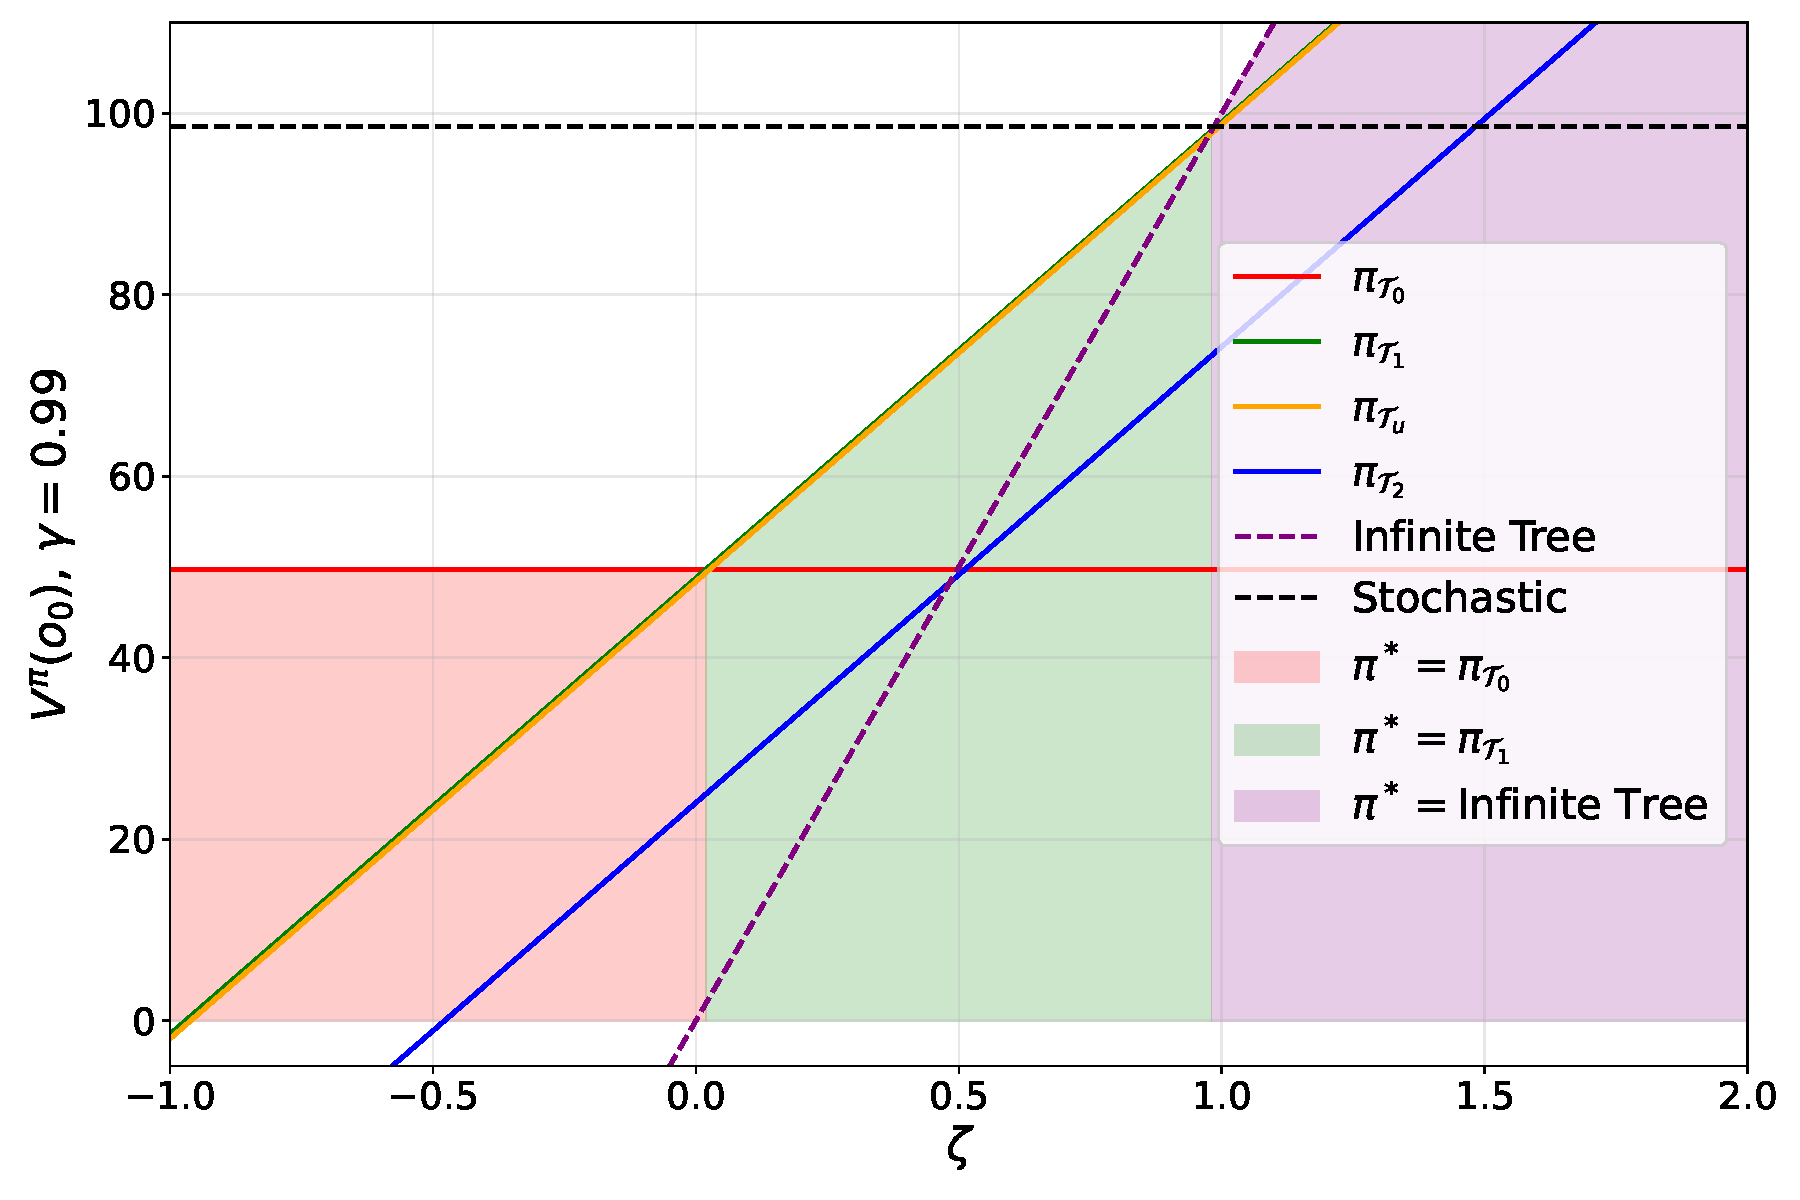
\includegraphics[width=1\textwidth]{images/images_part1/objective_values_plot.pdf}
    \caption{IBMDP objective values.}\label{fig:objectives}
\end{figure}
\section{Results}
\begin{figure}
    \centering
    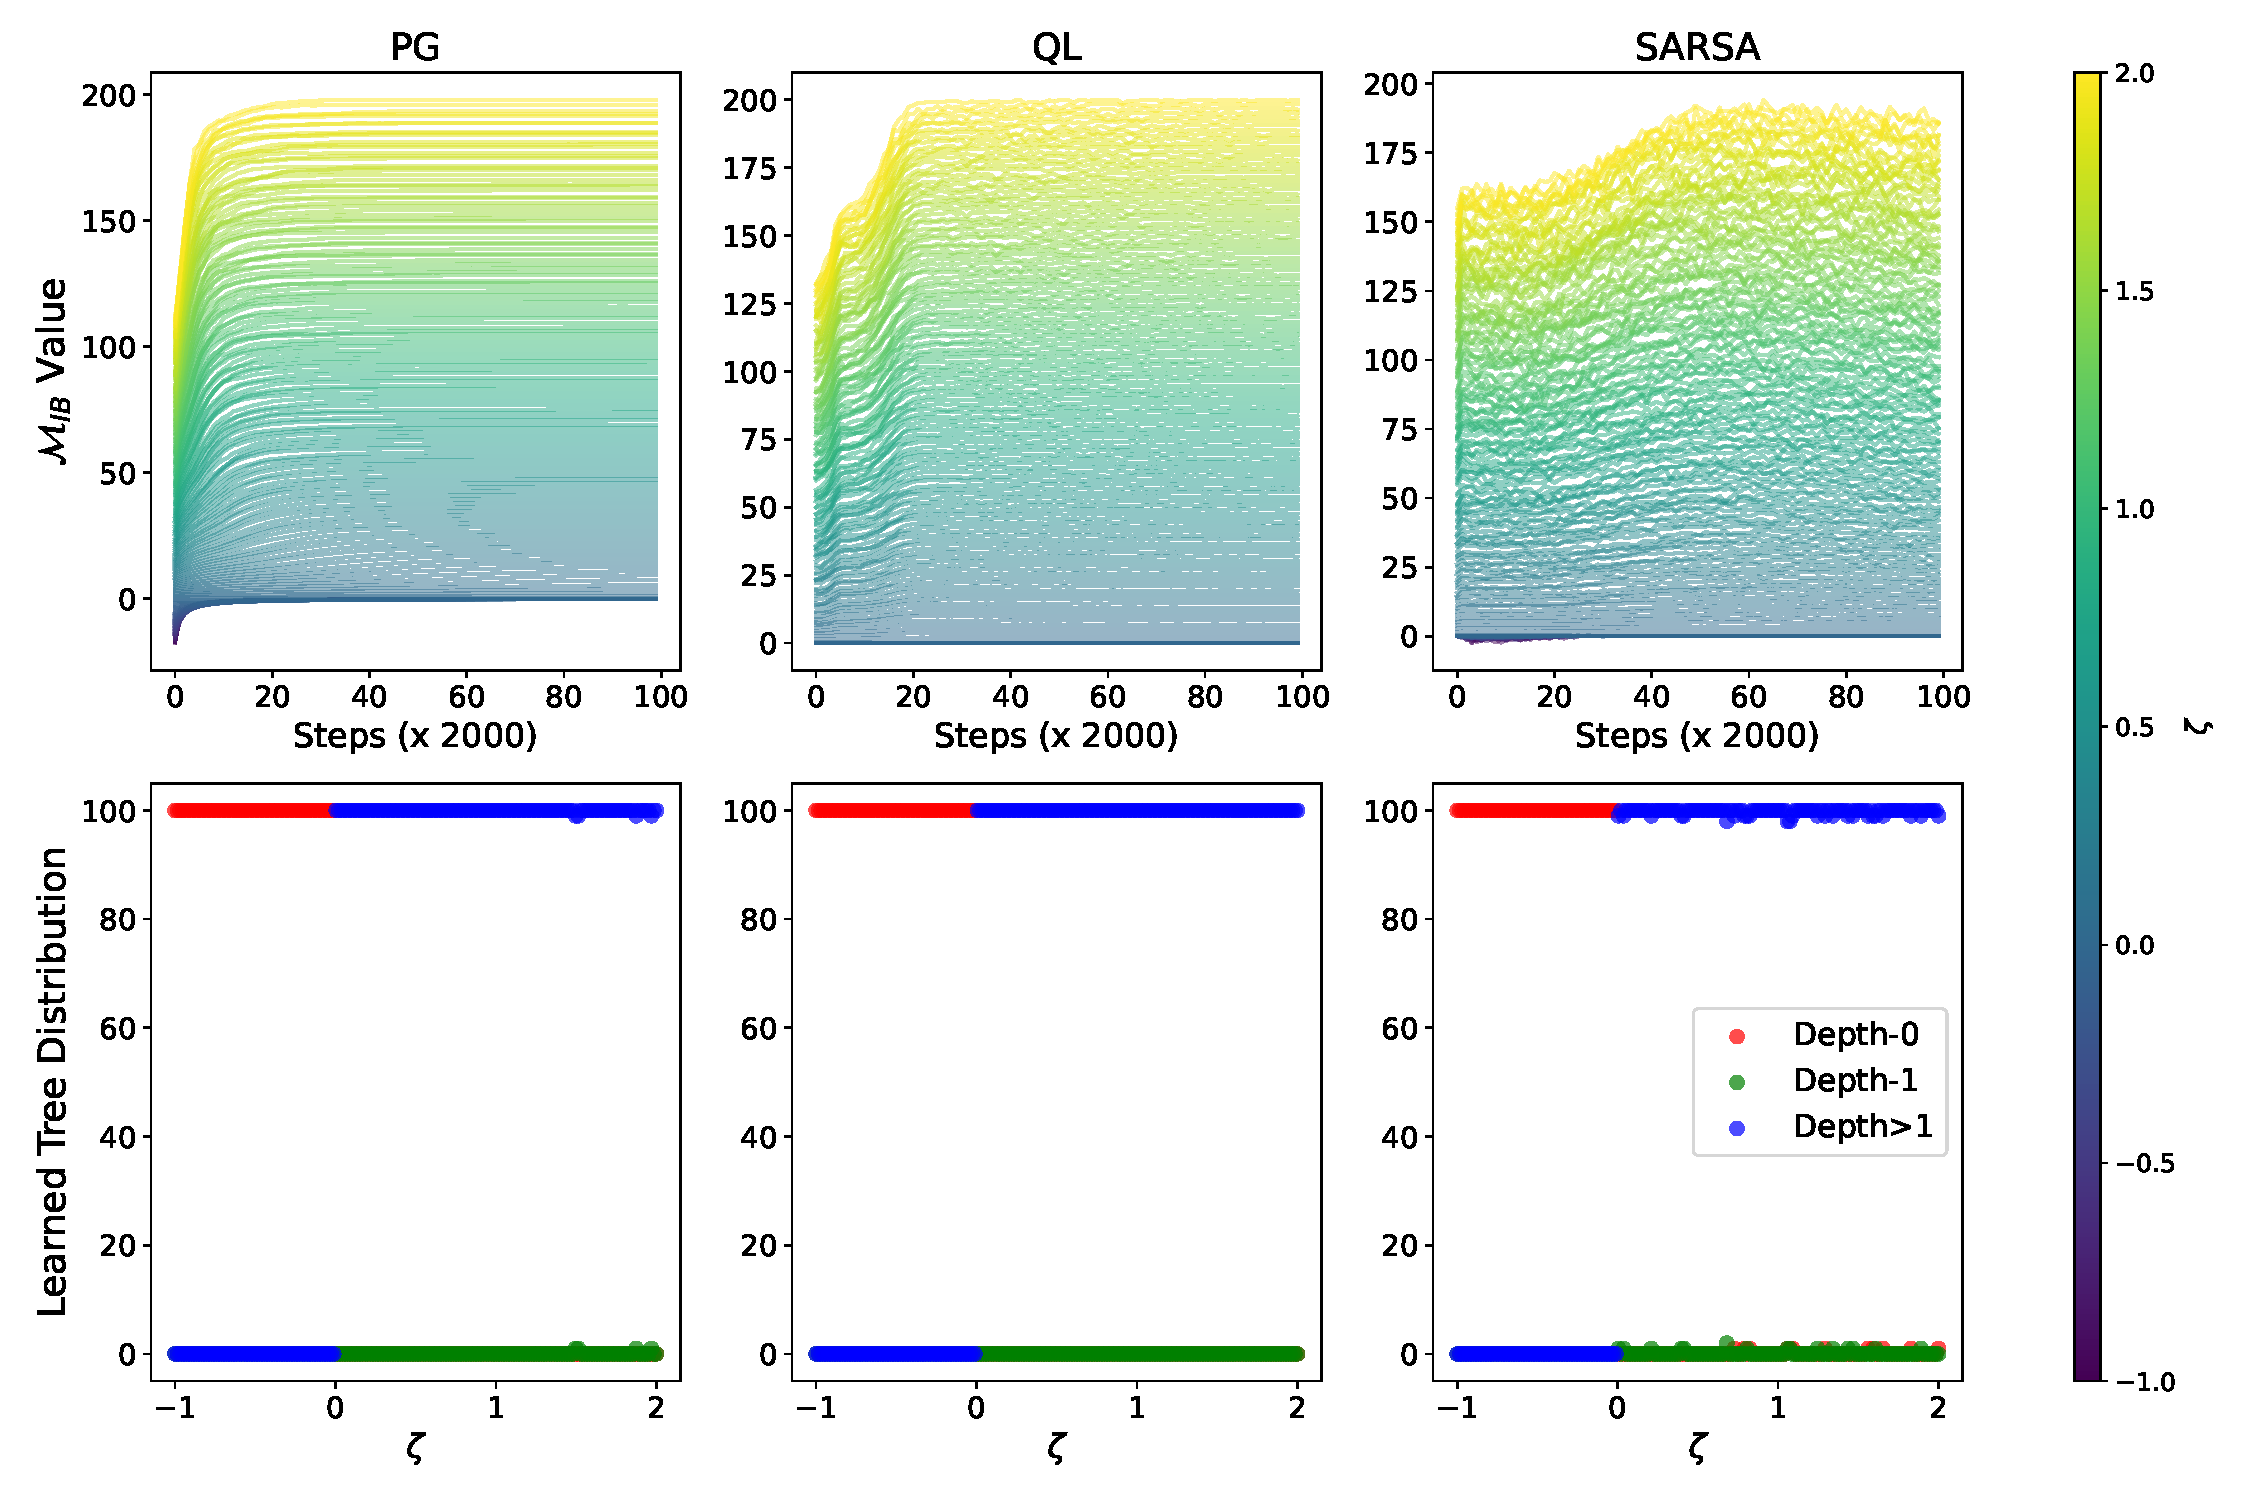
\includegraphics[width=1\textwidth]{images/images_part1/quick_plot_combined.pdf}
    \caption{RL algorithms for POIBMDPs}\label{fig:rl-poibmdp}
\end{figure}
\begin{figure}
    \centering
    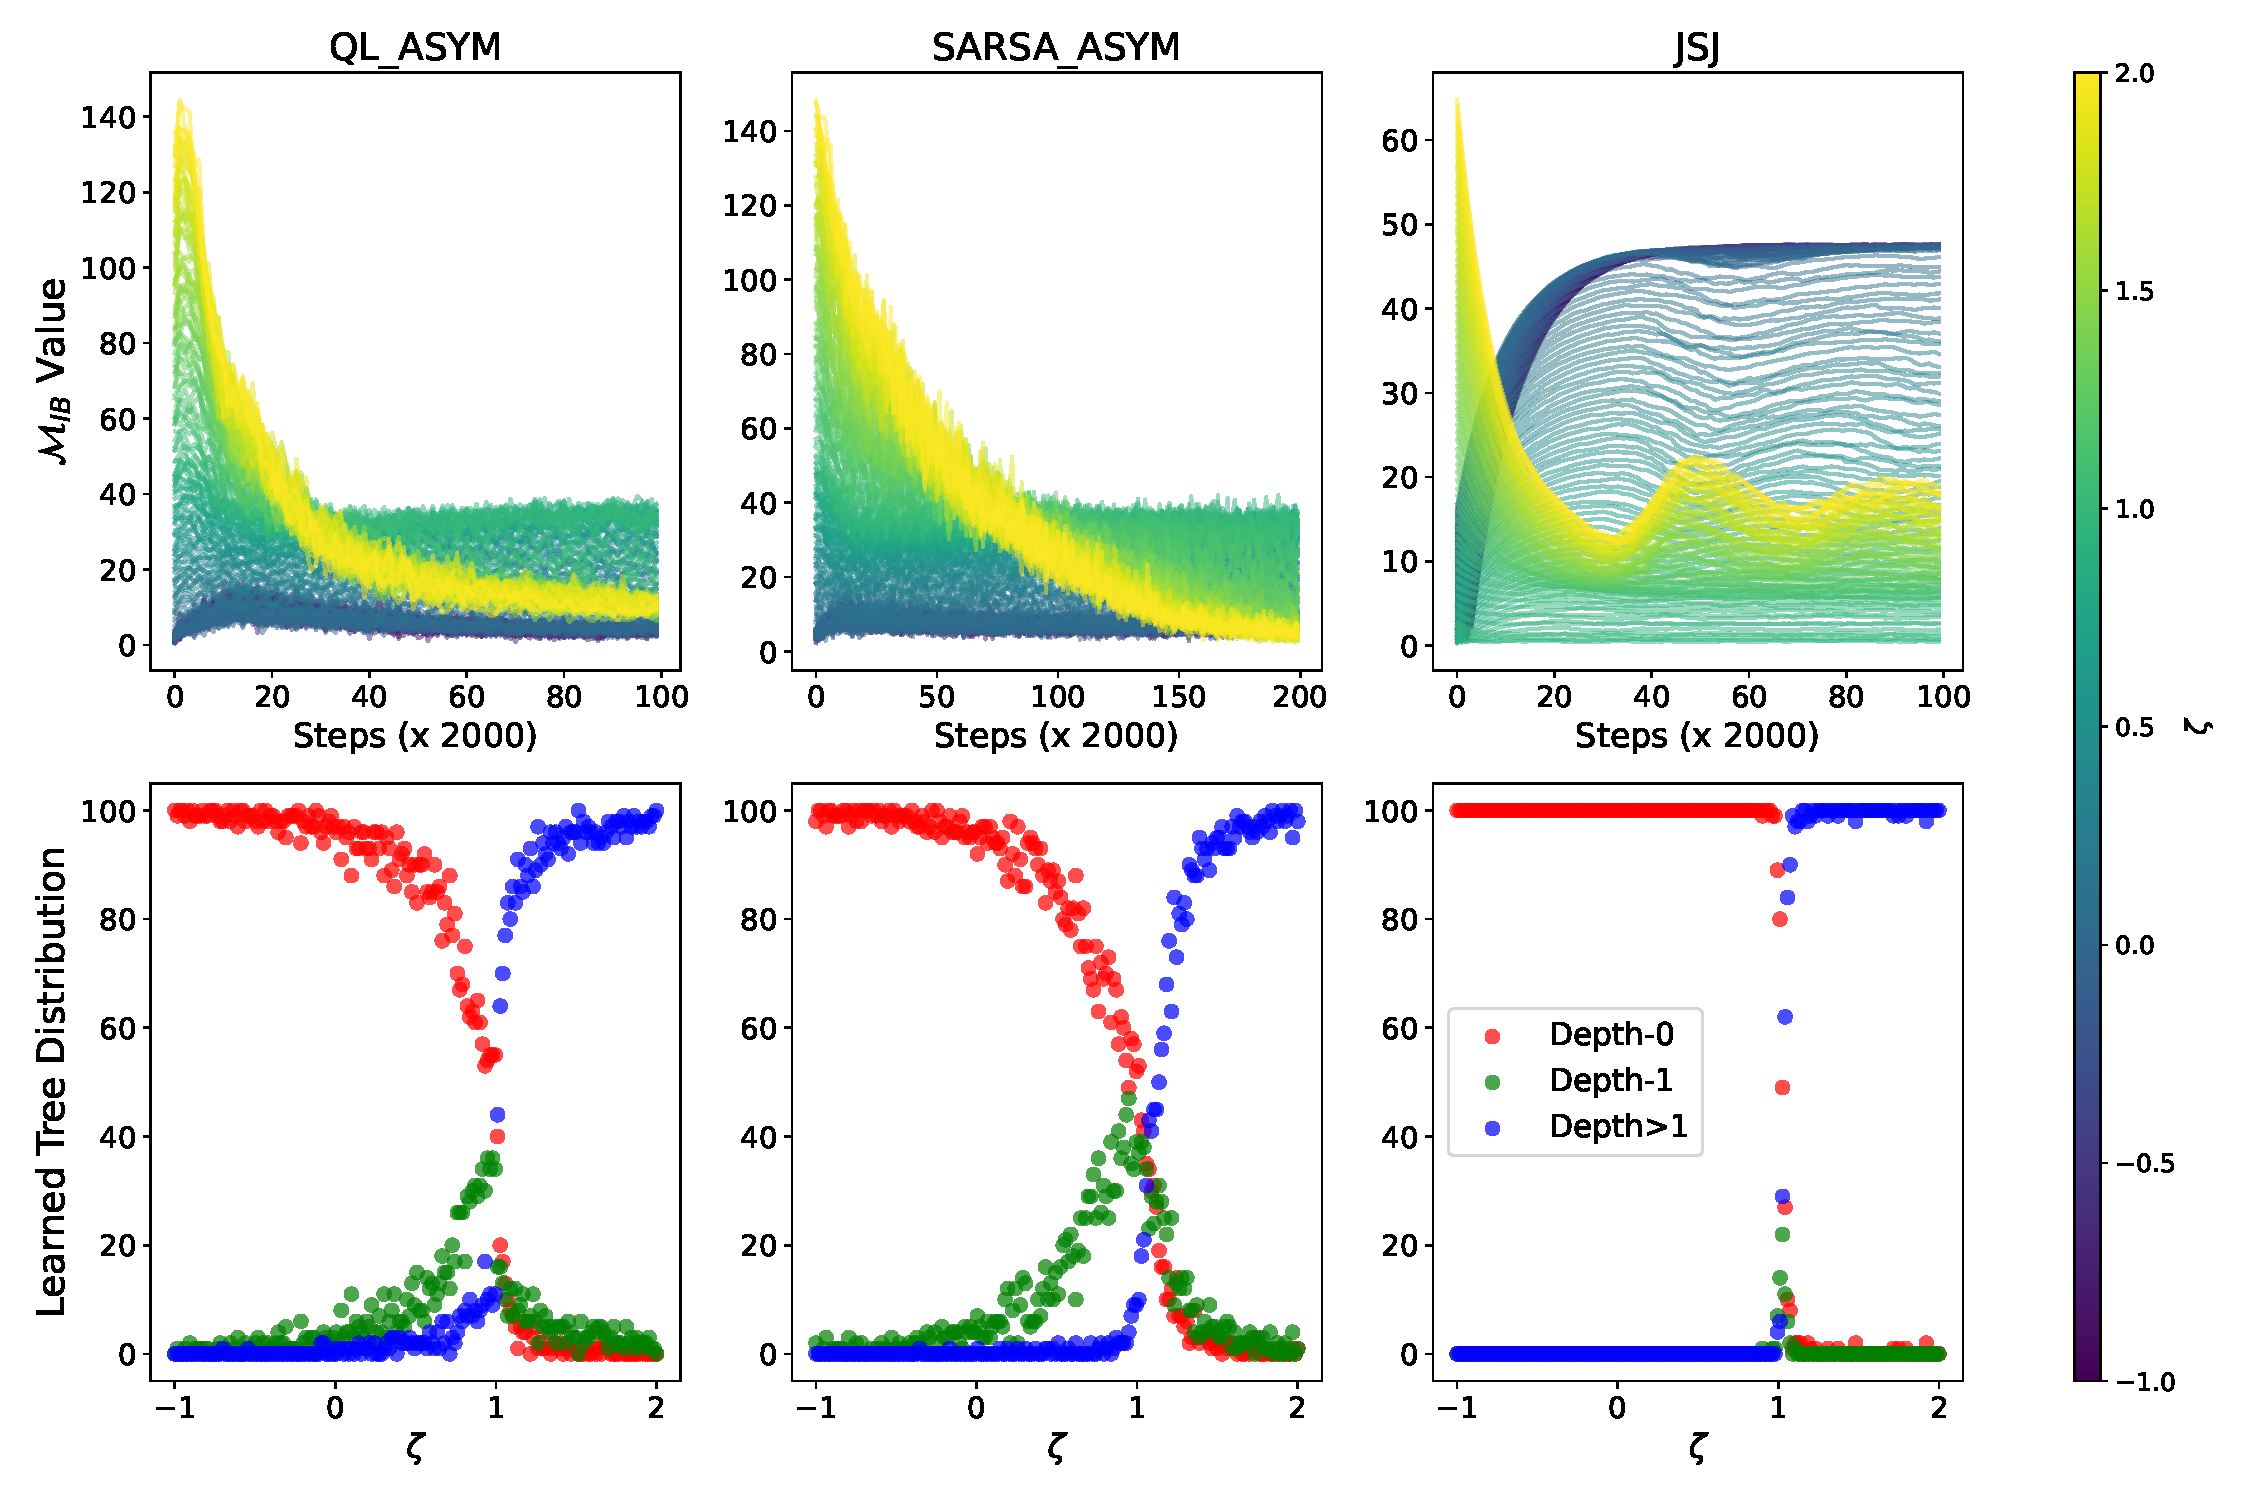
\includegraphics[width=1\textwidth]{images/images_part1/quick_plot_combined_po.pdf}
    \caption{Special algorithms for POIBMDPs}\label{fig:asym-rl-poibmdp}
\end{figure}
\begin{figure}
    \centering
    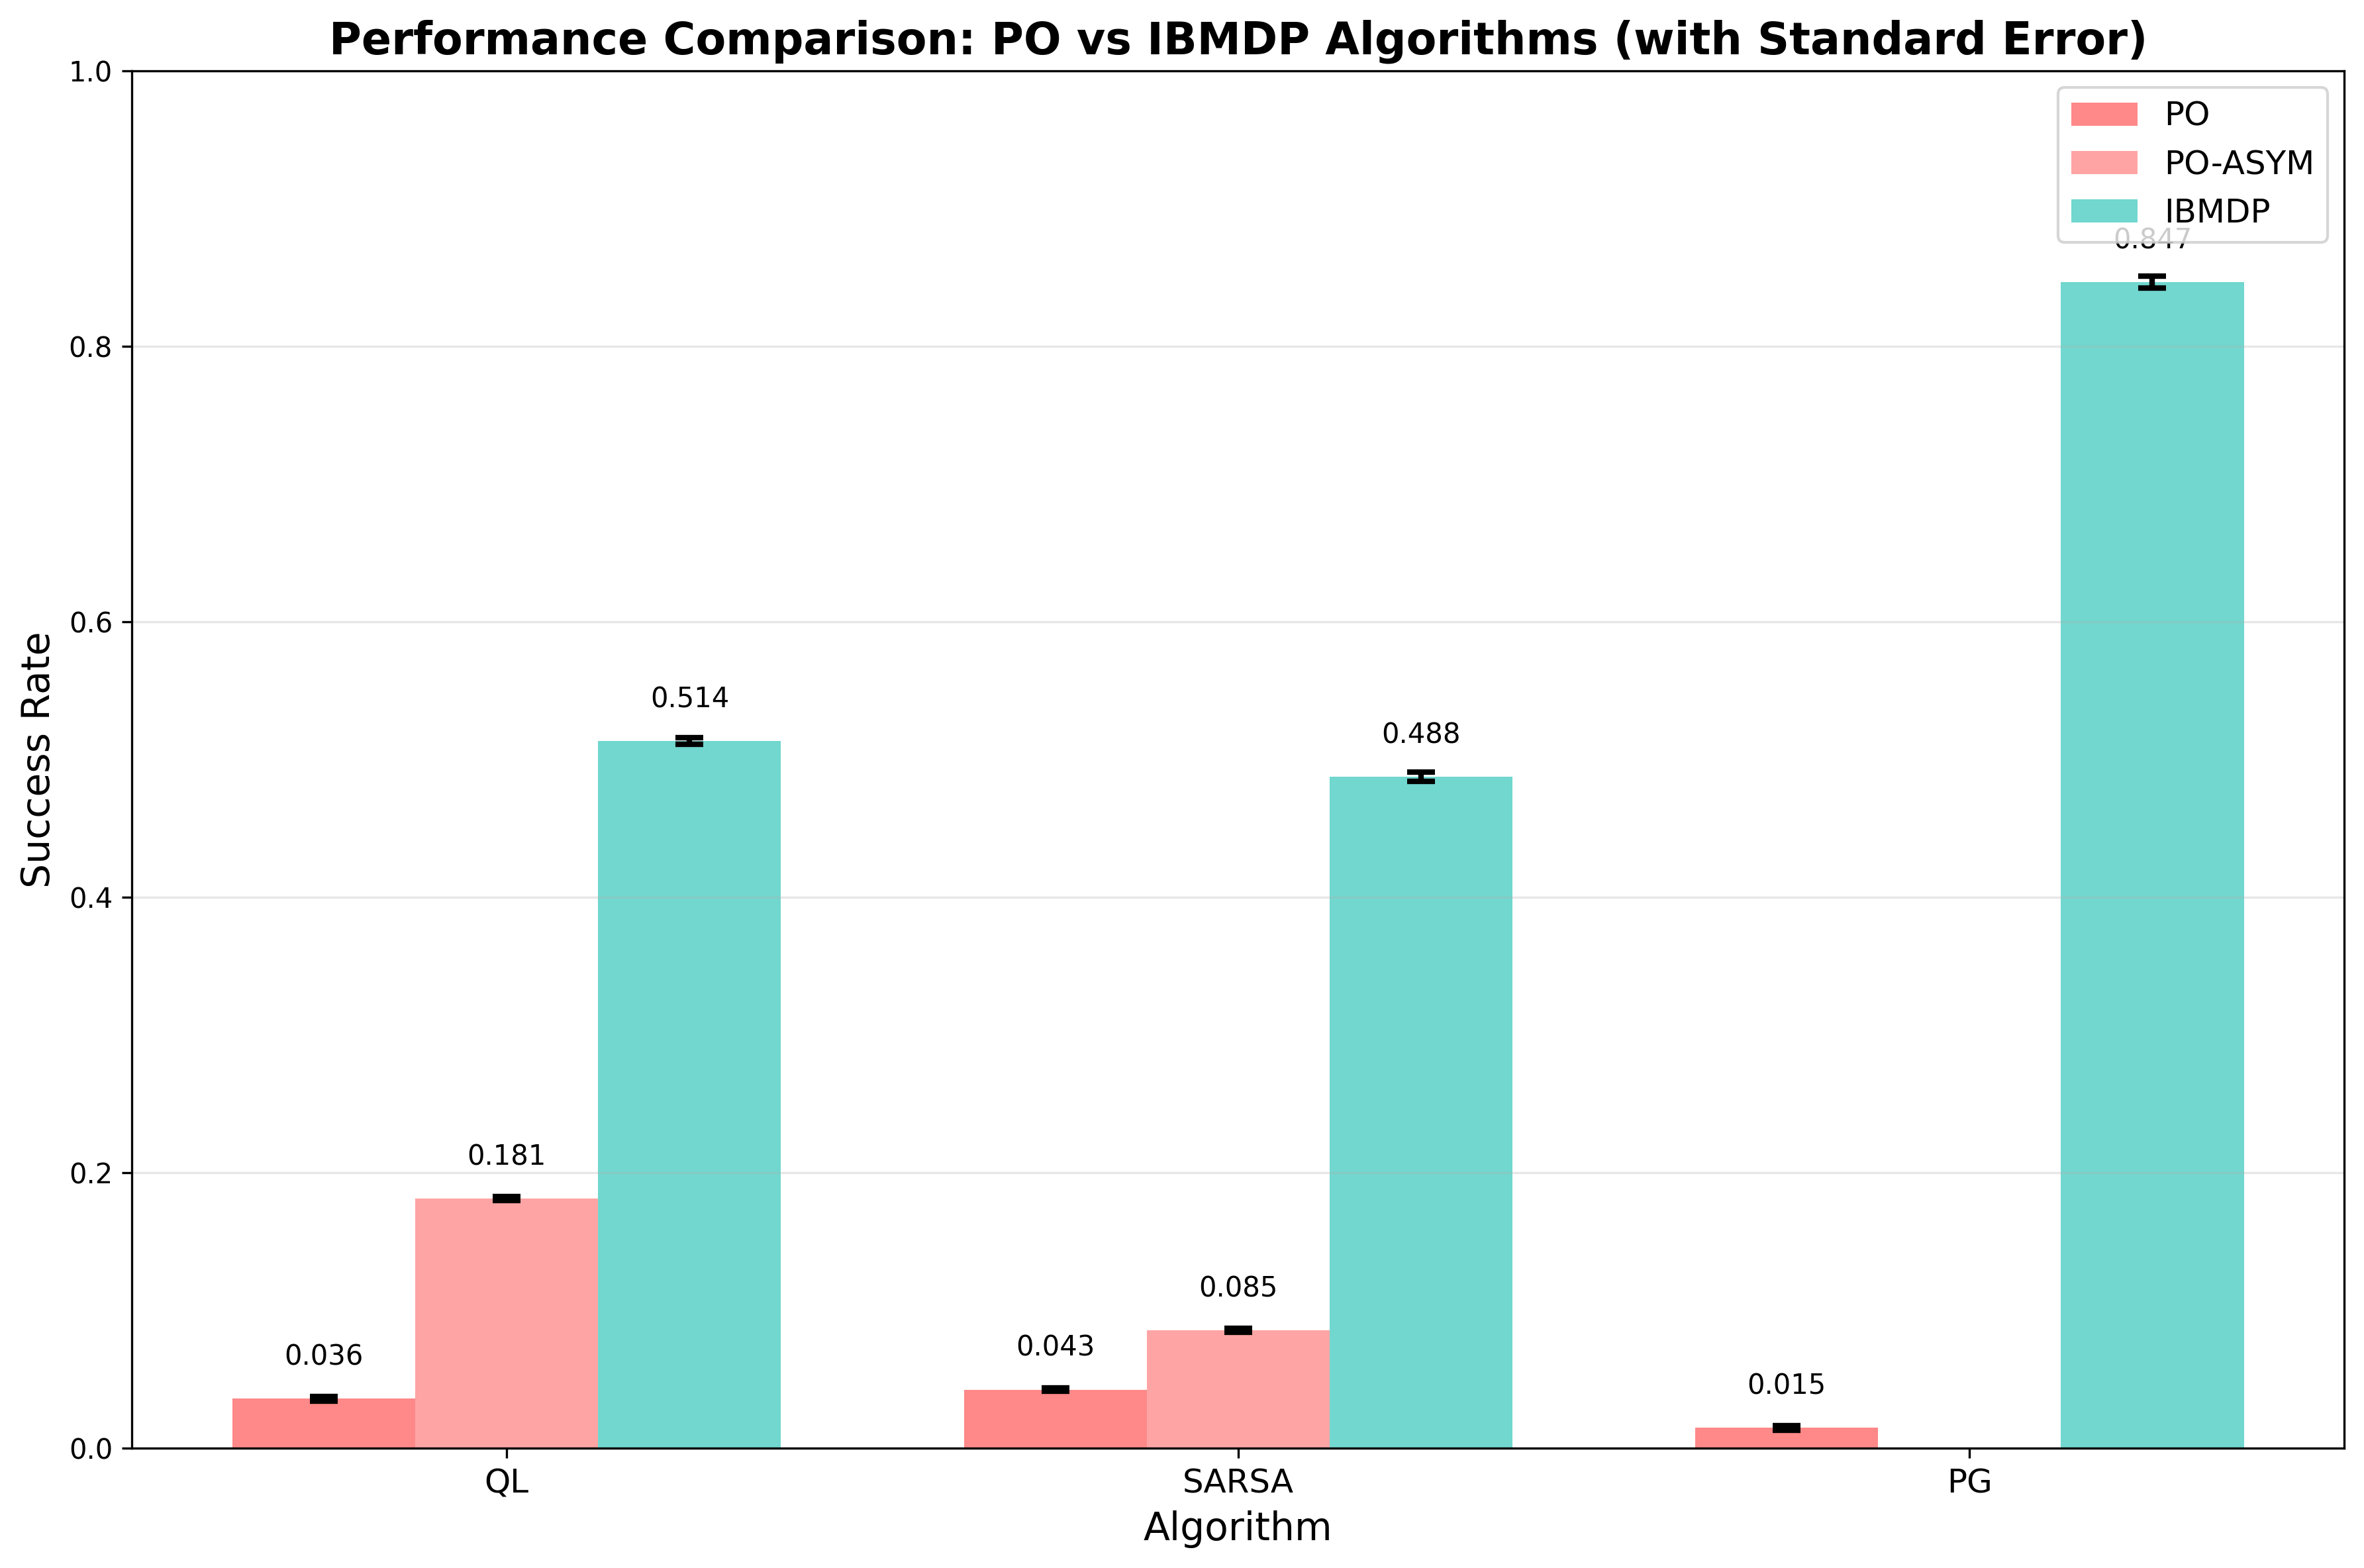
\includegraphics[width=1\textwidth]{images/images_part1/algorithm_performance_comparison_with_errors.png}
    \caption{PO vs IBMDPs}\label{fig:po-vs-ib}
\end{figure}
